\documentclass{beamer}
\usepackage{amsmath}
\usepackage{amssymb}
\usepackage{gvv}
\usepackage{bm}
\usepackage{graphicx}

\usetheme{Madrid}
\usecolortheme{default}

\title{\textbf{5.2.8}}
\author{\textbf{Aditya Mishra-EE25BTECH11005}}
\date{October 2, 2025}

\begin{document}

\begin{frame}
\titlepage
\end{frame}

\begin{frame}{Question}
Solve the equations:
\[
\begin{cases}
5x - 3y = 11 \\
-10x + 6y = -22
\end{cases}
\]
\end{frame}

\begin{frame}{Forming Augmented Matrix}
\[
\augvec{2}{1}{5 & -3 & 11 \\ -10 & 6 & -22}
\]
\end{frame}

\begin{frame}{Row Operations}
\[
\augvec{2}{1}{5 & -3 & 11 \\ -10 & 6 & -22}
\xrightarrow{R_2 \rightarrow R_2 + 2R_1}
\augvec{2}{1}{5 & -3 & 11 \\ 0 & 0 & 0}
\]

The second row turns out to be all zeros, meaning the system is dependent and consistent.
\end{frame}

\begin{frame}{Solution}
From the first row:
\[
5x - 3y = 11 \implies x = \frac{11 + 3y}{5}
\]

Let \(\vec{y} = \lambda, \lambda \in \mathbb{R}\) \
Then, the general solution is:
\[
\vec{x} = \myvec{\frac{11}{5} \ 0} + \lambda \myvec{\frac{3}{5} \ 1}, \quad \lambda \in \mathbb{R}
\]
\end{frame}

\begin{frame}{Plot}
\begin{figure}
    \centering
    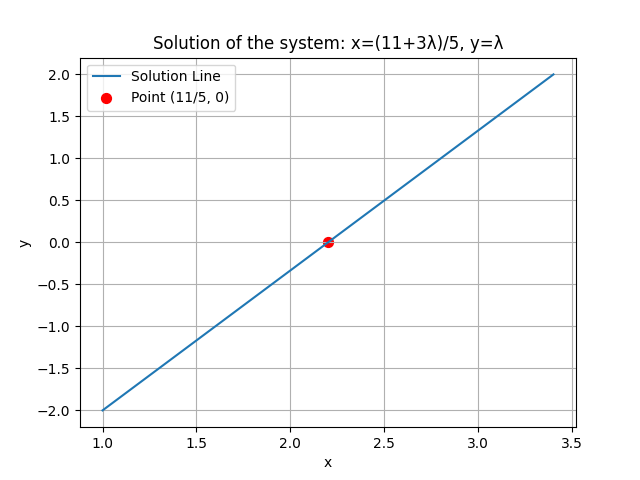
\includegraphics[width=0.8\columnwidth]{Figs/Figure_1.png}
\end{figure}
\end{frame}

\begin{frame}{Codes}
\centering
For Codes, refer to the URL below:  
\url{https://github.com/Aditya-Mishra11005/ee1030-2025/tree/temp/ee25btech11005/matgeo/5.2.8/Codes}
\end{frame}
\end{document}

